\chapter{Szenarios}

\section{ARP-Spoofing}

\section{DNS-Spoofing}

\subsection*{Vorraussetzungen}

\begin{itemize}
\item Kali Linux 2.0
\item ARP-Spoofing
\item dnsspoofing
\end{itemize}


\subsection*{Grundlagen}

\subsubsection*{DNS}
Die Addressierung und der anschließende Verbindungsaufbau zu einem Server erfolgt über eine eindeutige IP-Adresse. Damit der Mensch leichter eine Verbindung zu einem Server aufbauen kann,
wurde das DNS (Domain Name System) eingeführt. Dieses verwendet so genannte Domains zur Idenitifzierung von Servern, beispielweise "www.thi.de", da sich diese leichter merken lassen, als
eine IP-Adresse (z.B. 194.94.240.179). DNS ähnelt damit der Funktionsweise eines Telefonbuchs.
Das Domain Name System ist baumförmig aufgebaut, wie nachfolgende Abbildung \ref{fig:dns} illustriert: \\
\begin{figure}[h!]
	\centering
	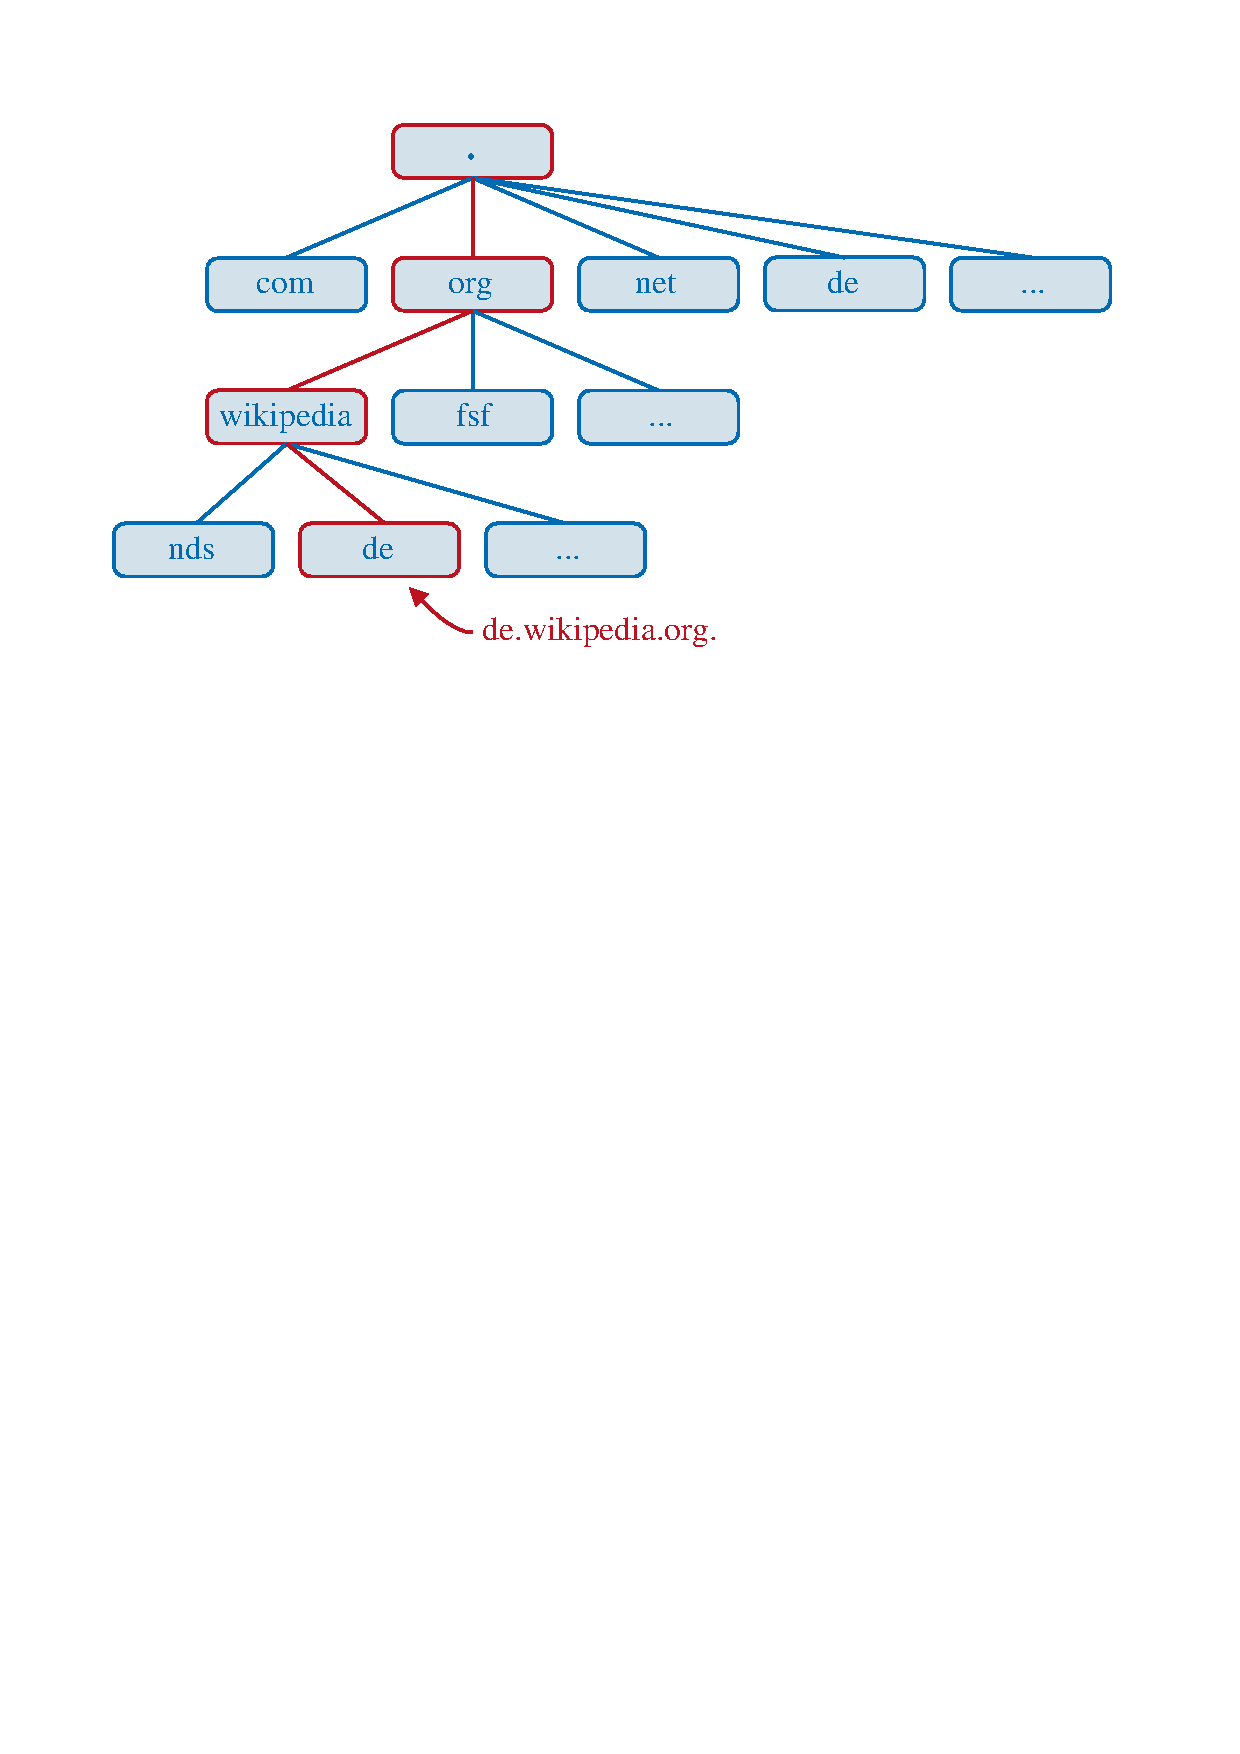
\includegraphics[width=0.7\textwidth]{bilder/dns.pdf}
	\caption{Aufbau DNS \cite{dnspicture}}
	\label{fig:dns}
\end{figure}

%[https://de.wikipedia.org/wiki/Domain_Name_System#/media/File:Dns-raum.svg]


\subsection*{Szenario}
Ein Client (z.B. Windows-Rechner) möchte die Internetseite der Technischen Hochschule Ingolstadt (www.thi.de) aufrufen. Dazu stellt dieser einen DNS-Request an seinen lokalen DNS-Server.
Wenn dieser in seinem Cache keinen Eintrag findet, frägt er - beginnend am Root-DNS-Server - iterativ alle Nameserver nach ihren Einträgen ab, um zum Schluss die IP-Adresse von www.thi.de
zu erhalten.\\
\begin{figure}[h!]
	\centering
	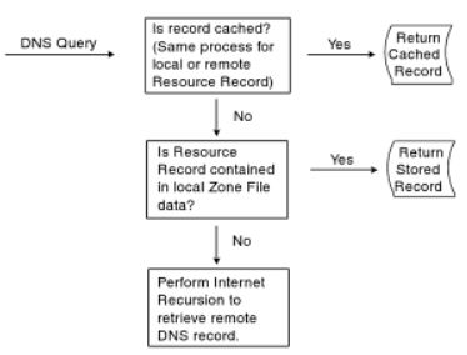
\includegraphics[width=0.7\textwidth]{bilder/DNS-Request.pdf}
	\caption{Ablauf DNS-Anfrage \cite{young2003hacker}}
	\label{fig:dnsrequest}
\end{figure}
%Abbildungs-Quelle: The Hacker's Handbook: The Strategy Behind Breaking into and Defending Networks - Seite 335

\subsection*{Technisches}
Um einen DNS-Eintrag für eine Domain, beispielsweise www.thi.de, zu manipulieren, kann mittels DNS Cache Poisoning der lokale DNS-Cache des Clients mit falschen Einträgen "vergiftet" werden.
Da bei jeder DNS-Anfrage eine zufällig generierte Transaktions-ID mitgeschickt wird, und eine DNS-Antwort nur akzeptiert wird, wenn diese mit der Anfrage übereinstimmt, muss man als Angreifer diese ermitteln, was sich in einem lokalen Netzwerk mit einem Sniffer sehr einfach realisieren lässt. Alternativ kann auch die Transaktions-ID erraten werden, wofür für die 16-Bit lange Transaktions-ID im Durchschnitt 32.768 Versuche notwendig sind.

\subsection*{Tools}
DNSSpoofing wurde von Dug Song \footnote{Diese und weitere Tools von Dug Song sind unter \url{www.monkey.org/~dugsong/dsniff} erhältlich.} entwickelt und veröffentlicht. Mit Unterstützung dieses Tools ist ein Manipulation des DNS-Caches eines Clients im lokalen
Netzwerk sehr leicht durchzuführen. Das Tool ermittelt die verwendeten Transaktions-ID durch Sniffen der ID, wenn der DNS-Server versucht eine Antwort an den Client zu übermitteln. Sobald er die ID der
Anfrage ermittelt hat, muss er eine schnellere Antwort an den anfragenden Client versenden, als der eigentliche DNS-Server. Dies geschieht in mehrfachen Tests und Analysen durch Wireshark regelmäßig. \\

\subsection*{Benutzung von DNS-Spoofing-Skript}
Um dnsspoof einsetzen zu können, muss initial eine hosts-Datei erstellt werden, die die zu manipulierenden Einträge in folgendem Format enthält: \newline

\begin{lstlisting}[caption=Beispiel für eine Hosts-Datei]{Name}
<IP-Adresse>		<Domain>
<192.168.20.135>	www.thi.de
(Wichtig ist hierbei die Trennung von IP-Adresse und Domainname durch Tab und keinen Leerzeichen!)
\end{lstlisting}

Anschließend wird \textit{dnsspoof} mit folgenden Parameter aufgerufen: \newline

\begin{lstlisting}[caption=Parameter für dnsspoof]
	\item[-i] Interface in dem sich lokales Netzwerk befindet
	\item[-f] Hosts-File, absoluter Pfad zu Ort der erstellten hosts-Datei
\end{lstlisting}
	



\subsection*{Gegenmaßnahmen}

\subsubsection*{DNSSEC}
Durch DNSSEC kann die Authenzität einer DNS-Antwort verifiziert werden und somit DNS Cache Poisoning vorgebeugt werden. Durch eine asymmetrische Signatur -  ähnlich PGP - kann der Absender
der DNS-Antwort, also der DNS-Server, seine Antworten signieren, indem er mit dem nur ihm zugänglichen privaten Schlüssel den Record unterschreibt. Die Clientseite kann anschließend im 
Gegenzug die Antwort mit dem öffentlichen Schlüssel des DNS-Servers überprüfen, ob die Antwort auch von dem richtigen Server war.\newpage

\section{Denial of Service (DoS)}


\subsection*{Vorraussetzungen}

\begin{itemize}
\item Kali Linux 2.0
\item Python mit Socket- und Thread-Bibliothek
\end{itemize}


\subsection*{Grundlagen}

\subsubsection*{TCP}
TCP (Transmission Control Panel) ist ein verbindungsorientiertes Protokoll zur verlustfreien Übertragung von Daten und Datenströmen. Verschiedene Mechanismen sorgen dafür, dass Datenpakete zuverlässig und verbindungsorientiert übertragen werden.

\subsection*{Szenario}

DoS (Denial of Service, zu dt: Dienstblockade) bezeichnet die vorübergehende Nichtverfügbarkeit eines Dienstes, durch Überlastung. Wird die Überlastung von mehreren Systemen verursacht,
spricht man von DDoS (Distributed Denial of Service). \\
Bei einem DoS-Angriff mittels SYN-Flooding wird das Übertragungsprotokoll TCP verwendet, da es zustandsorientiert ist, und somit der angesprochene Server Ressourcen für den Anfragenden reserviert.
 Das Aufrechterhalten der Ressourcen wird durch eine fehlende ACK-Bestätigung des Clients realisiert, nachdem der Server vorher ein SYN-ACK-Bestätigung übermittelt hat. Durch Versenden von sehr vielen SYN-Paketen auf den selben Zielserver kann es vorkommen, dass auf dem angegriffenen Server keine Ressourcen mehr vorhanden sind, um weitere Anfragen annehmen zu können. Die dann folgenden Pakete werden vom Server umgehend verworfen und es kann keine Verbindung aufgebaut werden. \cite{dnssec}

\subsection*{Technisches}
Das selbst geschriebene Python-Skript versendet eine vorgegebene Anzahl von SYN-Paketen an eine Zieladresse. Durch einen Iptables-Eintrag wird verhindert, dass nach Erhalt der SYN-ACK-Bestätigung
des Zielserveres eine ACK-Bestätigung zurückgeschickt wird. Dadurch wird für eine bestimmte Zeit Ressourcen reserviert, die in Summe zur Überlastung des Servers führen.

\subsection*{Tools}
-> siehe Technisches

\subsection*{Benutzung von DoS-Skript}
Das Skript frägt interaktiv den Benutzer alle erforderlichen Angaben ab. Diese sind die Anzahl der SYN-Pakete und die IP-Adresse des Zielservers.

\subsection*{Gegenmaßnahmen}

\subsubsection*{Netzwerk Monitoring}
Mittels eines Intrusion Detecten (IDS) und Prevention System (IPS) kann die Aktivität und der Ursprung eintreffender SYN-Pakete analysiert werden und beispielsweise nur eine bestimmte Anzahl von Paketen pro
Minute zugelassen werden. Sollten von der Quell-IP-Adresse dann noch weitere Pakete eintreffen, werden diese bereits an der Firewall verworfen. \footnote{Mehr Informationen zu Umfang und Möglichkeiten von IDS und IPS finden Sie unter folgendem Paper:\cite{differenceipsids}} 

\subsubsection*{SYN-Cookies}
Mittels SYN-Cookies kann bei Verbindungsaufbau durch den Server überprüft werden, ob der Client bereits versucht hat, eine Verbindung herzustellen. Bei Implementierung von SYN-Cookies reserviert der Server keine Ressourcen bei Eintreffen eines SYN-Paketes von einem Client, sondern speichert nur einen Hashwert mit Informationen des SYN-ACK-Paketes. Wenn der Client im dritten Schritt ein SYN-Paket mit der Bestätigung des SYN-ACKs an den Server übermittelt hat, wird mittels des gespeicherten Hashwertes überprüft, ob dieser Client bereits vorher mit dem Server kommuniziert hat. Falls diese Überprüfunge positiv ausfällt, wird eine TCP-Verbindung aufgebaut.\newpage


\section{SSL-Strip}

\subsection*{Vorraussetzungen}

\begin{itemize}
\item Kali Linux 2.0
\item IP Forward
\item IPtables
\item ARP-Spoofing
\item SSLStrip
\end{itemize}


\subsection*{Grundlagen}

\subsubsection*{HTTP}
HTTP (Hypertext Transfer Protocol) ist ein zustandsloses Protokoll zur Übertragung von Dokumenten auf Anwendungsschicht (siehe ISO-OSI-Layer). Der Standard wurde 1991 von der Internet Egnineering
Task Force (IETF) und dem World Wide Web Consortium (W3C) eingeführt und ist mittlerweile in Version 2.0 (HTTP/2) veröffentlicht. [1]
Nachfolgendes Schema (Abbildung x) verdeutlicht den Ablauf.

Meist wird HTTP verwendet um HTML-Seiten in Webbrowsern darzustellen.

\subsubsection*{HTTPS}
HTTPS (Hypertext Transfer Protocol Secure) wird dazu verwendet um Dokumente auf Anwendungsschicht über ein sicheres Protokoll übertragen zu können. Syntaktisch ist es wie HTTP aufgebaut,
 wird jedoch um eine Verschlüsselung der Daten umgeben. Zur Verschlüsselung der Daten wird SSL (Secure Socket Layer) bzw. TLS (Transport Layer Security) verwendet.

\subsubsection*{ARP}
siehe Eintrag Address-Resolution-Protocol

\subsection*{Szenario}
Eine MITM-Attacke auf eine verschlüsselte HTTPS-Verbindung ist nur mit sehr viel Rechenkapazität zu entschlüsseln. Eine einfachere Möglichkeit des Mitschneiden von übertragenen Datenpaketen ist die Verwendung einer unverschlüsselten HTTP-Verbindung. Da ein Großteil der Benutzer einen Unterschied von \textit{https://www.url.de} zu \textit{http://www.url.de} in der URL-Leiste kaum erkennen würden, ist SSLStrip eine gute Möglichkeit Datenpakete mitlesen und verändern zu können. \newline
Das Auslesen von Passwörtern für Online-Banking oder Webmail wären potentielle Ziele eines solchen Angriffs.

\subsection*{Technisches}
SSLStrip \footnote{ Dieses Tool kann über folgende Links abgerufen werden: \url{https://github.com/graingert/sslstrip/}, \url{http://www.thoughtcrime.org/software/sslstrip/}} wurde von Moxie Marlinspike 2009 entwickelt und ist aktuell in Version 0.9.2 verfügbar. Das Tool durchsucht jeden transparenten HTTP-Verkehr nach https-Links und wandelt diese in http-Links um. Um die Attacke durchführen zu können, wird zusätzlich ARP-Spoofing benötigt. Mittels ARP-Spoofing werden auch die unverschlüsselten HTTP-Links über SSLStrip verschickt. Da mittlerweile viele Webseiten (z.B. Online-Banking, Webmail, ...) nur noch verschlüsselte HTTP(S)-Verbindungen zulassen, baut SSLStrip eine verschlüsselte Verbindung zu diesen Seiten auf, und gibt deren Antwort in einer unverschlüsselten Verbindung an den kompromittierten Client zurück. Folgende Abbildung zeigt den Ablauf der HTTP(S)-Verbindungen zwischen einem Client, Angreifer und dem aufgerufenen (Web-)Server. \newpage

\begin{figure}[h!]
	\centering
	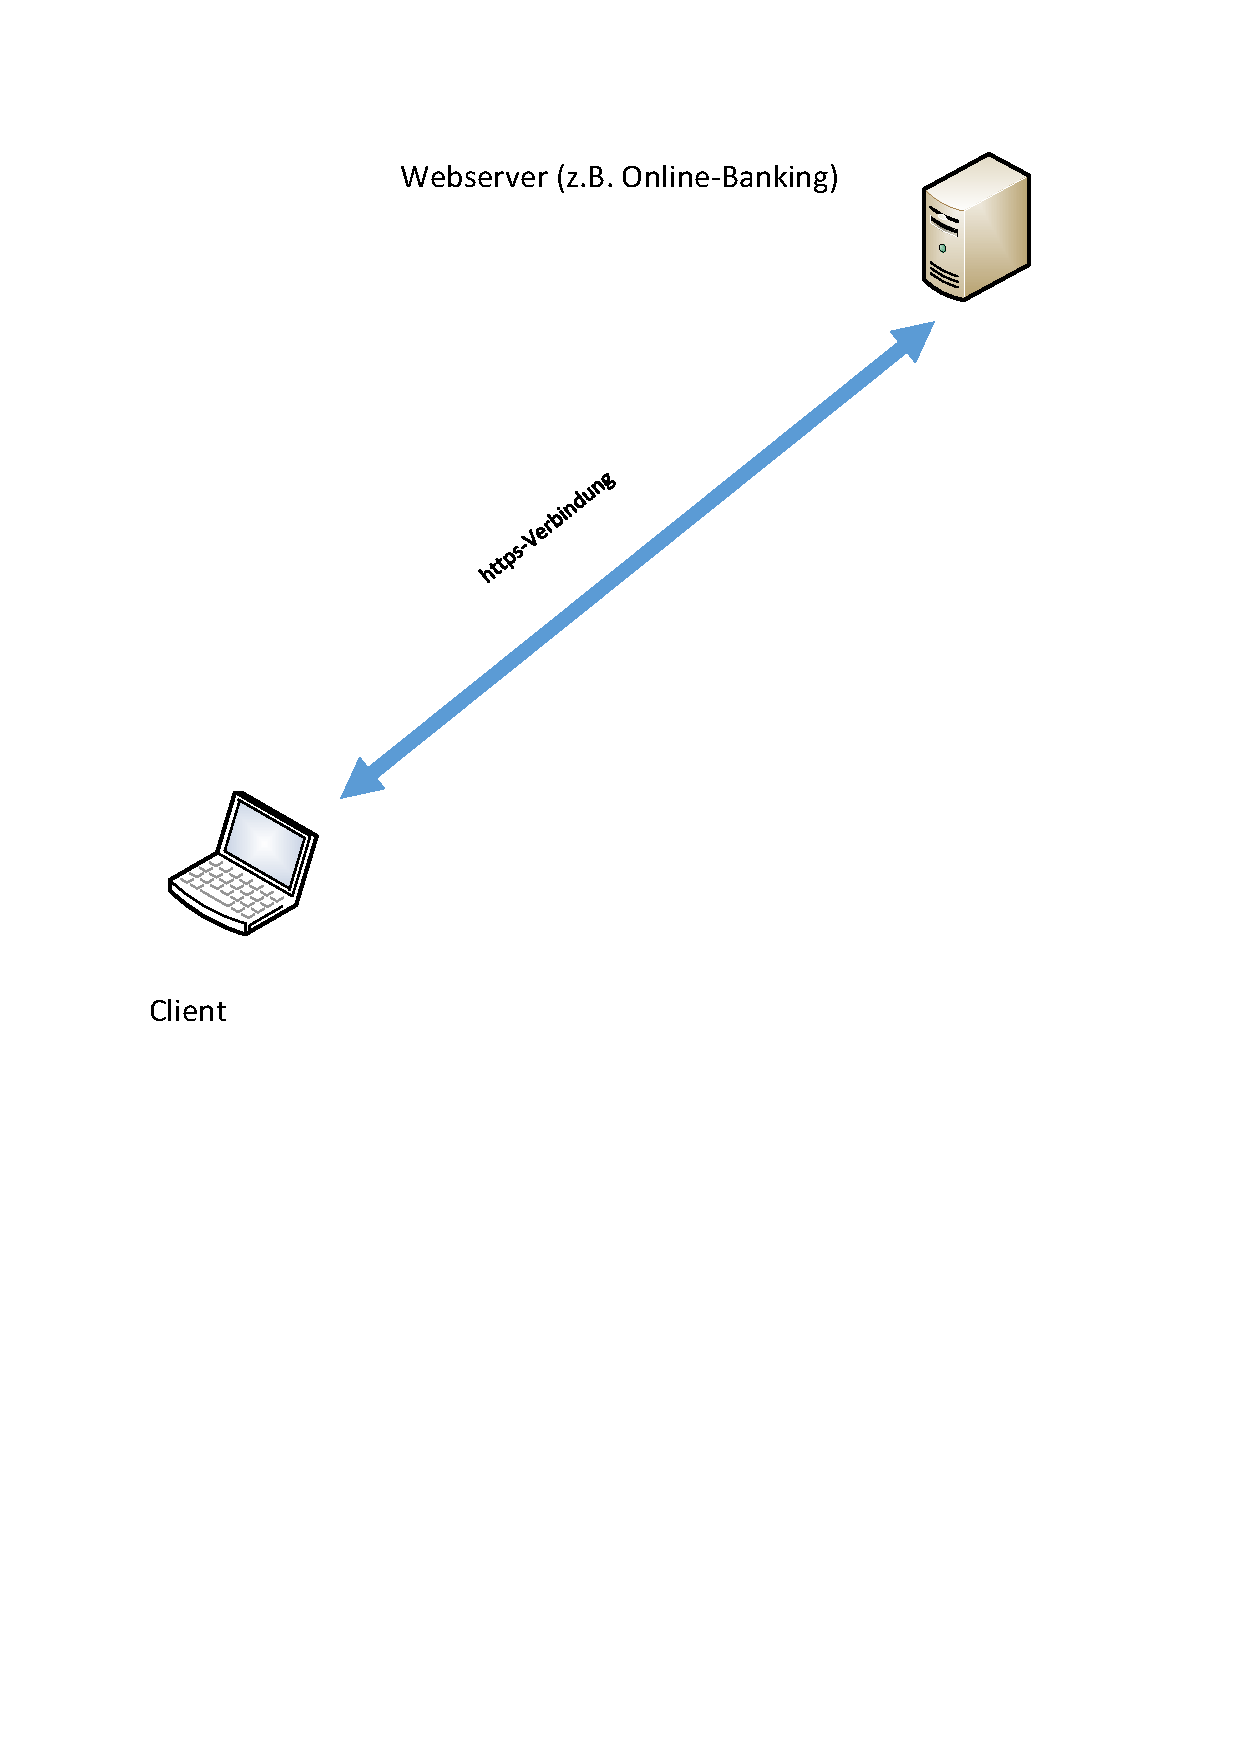
\includegraphics[width=0.6\textwidth]{bilder/https.pdf}
	\caption{Reguläre HTTPS-Verbindung zwischen Client und Server}
	\label{fig:https}
\end{figure}

\begin{figure}[h!]
	\centering
	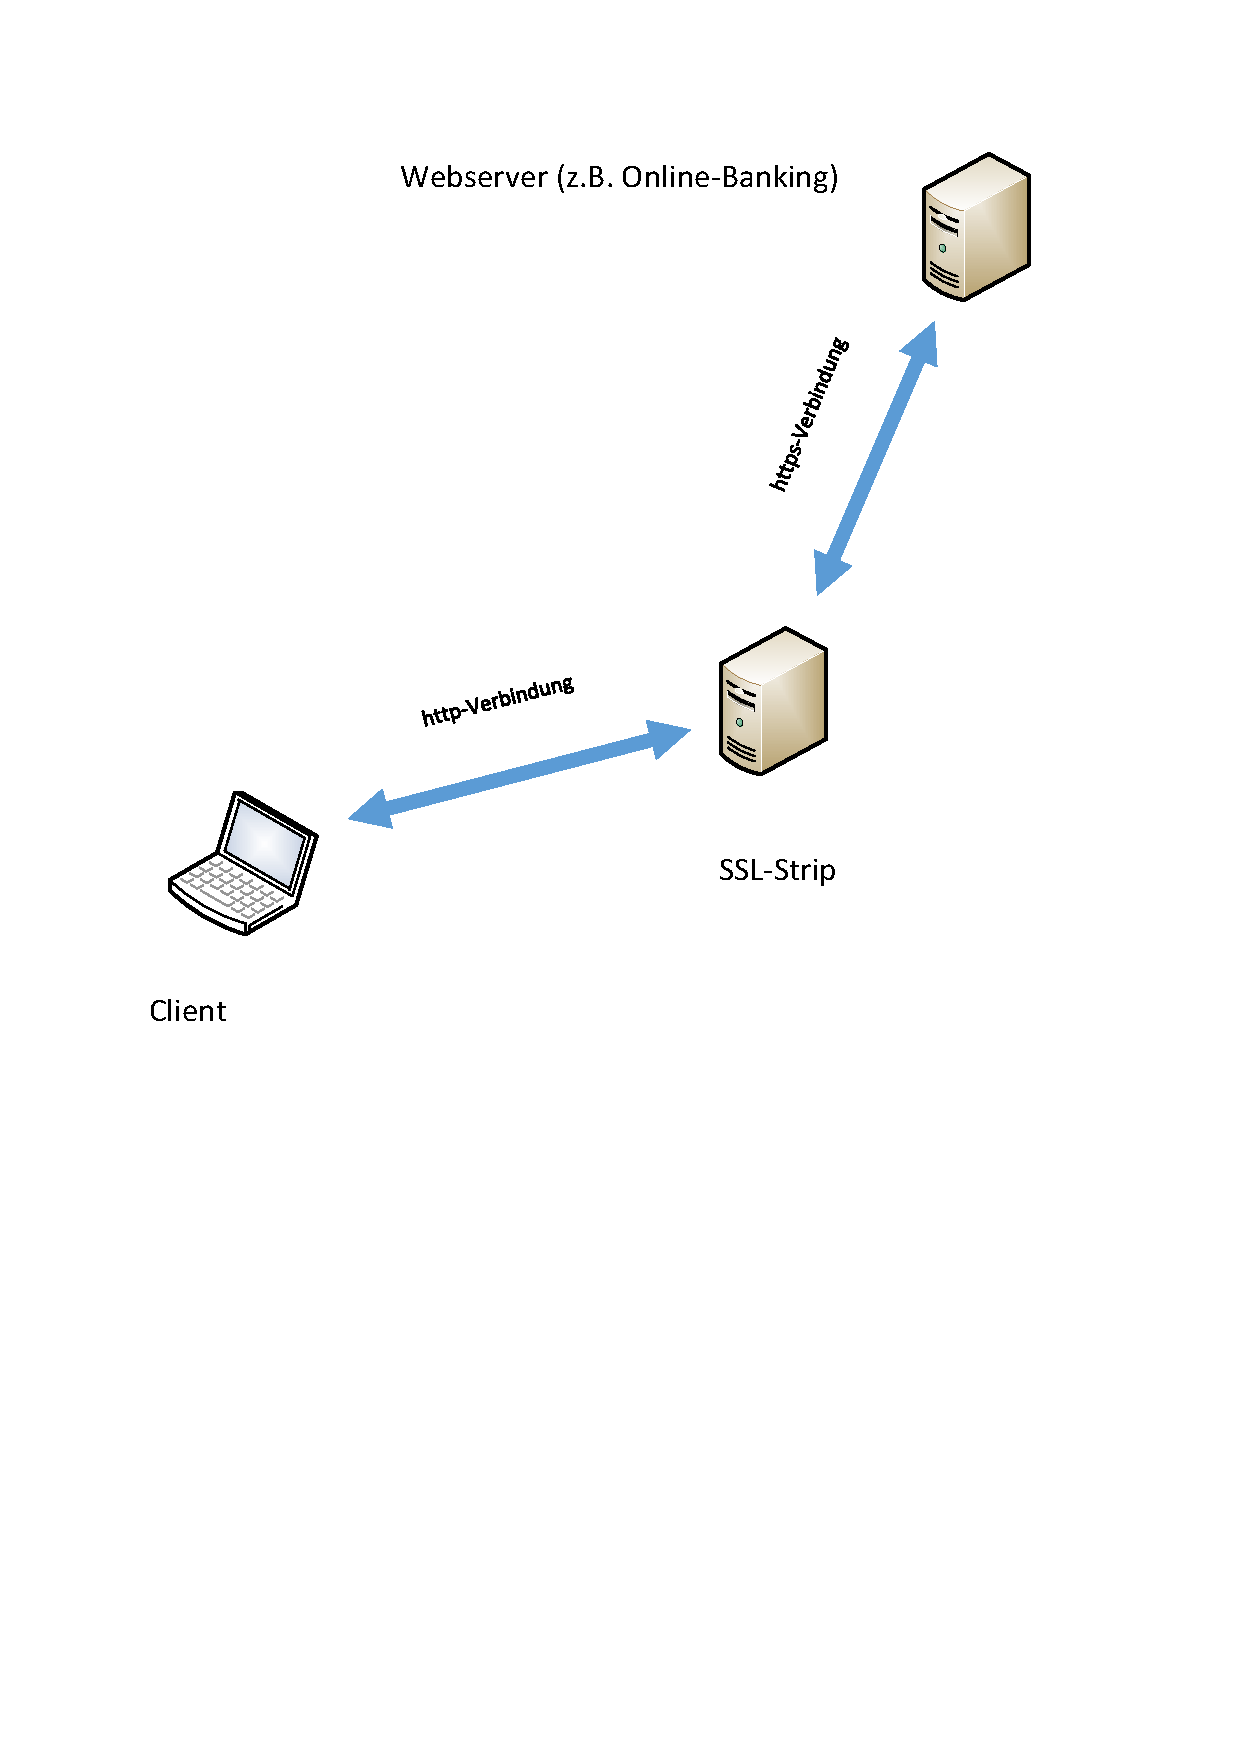
\includegraphics[width=0.65\textwidth]{bilder/sslstrip.pdf}
	\caption{SSL-Strip Szenario}
	\label{fig:sslstrip}
\end{figure}

\subsection*{Tools}
Um SSLStrip einsetzen zu können sind mehrere Schritte notwendig. Auf Kali Linux 2.0 sind alle benötigten Tools bereits vorinstalliert. \\

IP-Forwarding, also das Weiterleiten von IP-Paketen, kann durch folgende Befehle aktiviert werden:\\

\begin{lstlisting}[caption=Aktivieren von IP-Forwarding]{Name}
	sysctl -w net.ipv4.ip_forward=1
	alternativ: echo 1 > /proc/sys/net/ipv4/ip_forward
\end{lstlisting}
	

Anschließend wird ARP-Spoofing gestartet. Dies geschieht mit folgenden Befehlen:
\begin{lstlisting}[caption=Parameter für ARP-Spoofing]
arpspoof -i <interface> -t <targetIP> <gatewayIP>
Parameter:
	-i  <interface>		Angabe des Interfaces, in dem sich Angreifer und Client befinden.
	-t <targetIP>   	IP-Adresse des anzugreifenden Clients
	<gatewayIP>   		IP-Adresse des Gateways im LAN
\end{lstlisting}

Nachdem nun mittels ARP-Spoofing alle IP-Pakete vom angegriffenen Client über den Angreifer gesendet werden, müssen die umgeleiteten HTTP-Pakete via IPtables an das Tool SSLStrip weitergereicht werden. Dies geschieht mittels folgendem Eintrag:\\

\begin{lstlisting}[caption=Eintrag in IP-Tables damit HTTP-Pakete an sslstrip weitergereicht werden]
iptables -t nat -A PREROUTING -p tcp --destination-port 80 -j REDIRECT --to-port <listenPort>
Parameter:
	-t nat                 	: Firewall-Gruppe
	-A PREROUTING          	: Regel wird angewandt, BEVOR Paket geroutet wird
	-p tcp                 	: Nur TCP-Pakete
	--destination-port 80  	: Nur Pakete auf Port 80 (http)
	-j REDIRECT            	: Legt Aktion fest, also Weiterleitung
	--to-port <listenPort> 	: Port auf dem SSLStrip lauscht.
\end{lstlisting}


Nun muss noch SSLStrip selbst gestartet werden. Dies geschieht mittels folgender Eingabe:
\begin{lstlisting}[caption=Erforderliche Parameter für SSLStrip]
sslstrip -a -k -l <listenPort> -w <logpath>
Parameter:
	-s : Gesamter SSL Traffic wird gelogged
	-p : Nur SSL POST Traffic wird protokolliert
	-a : SSL- und HTTP-Traffic wird aufgezeichnet
	-k : Bestehende SSL-Verbindungen terminieren, damit diese neu aufgebaut werden
	-l : Port auf dem SSLStrip lauscht. Muss identisch zu --to-port bei iptables-Eintrag sein
	-w : Pfad in dem gehijackter HTTPS-Traffic im Klartext abgespeichert wird
\end{lstlisting}
	
\subsection*{Benutzung von SSLStrip-Skript}
Zur Automatisierung wurden vorangegangene Befehle in einem Skript automatisiert. Nachdem SSLStrip im Auswahlmenü selektiert wurde, wird zuerst nach der Netzwerkschnittstelle gefragt, in der Angreifer und Zielclient sich befinden. Anschließend wird das ausgewählte Netzwerk nach aktiven Hosts gescannt und aufgelistet. Im folgenden Schritt wird die Ziel-IP-Adresse des anzugreifenden Clients eingegeben, gefolgt von der IP-Adresse des Gateways für ARP-Spoofing. Abschließend werden die erforderlichen Konfigurationen für SSLStrip-Attacke im Hintergrund durchgeführt und der mitgeschnittene HTTPS-Verkehr im Klartext in der LOG-Datei abgerufen werden.
 
 
\subsection*{Gegenmaßnahmen}

\subsubsection*{HTTP Strict Transport Security}
HTTP Strict Transport Security ist ein Mechanismus um einem Client mitzuteilen, dass er für eine bestimmte Zeit nur verschlüsselte Verbindungen verwenden soll. Der Server übermittelt in seiner Antwort im Header, zusätzliche Informationen über die Gültigkeit der Information und ob sämtliche Subdomains ebenfalls ausschließlich verschlüsselte Verbindungen annehmen dürfen. \cite{hsts} \newpage
%Quellen:
%[1]https://de.wikipedia.org/wiki/Hypertext_Transfer_Protocol
%[2]https://de.wikipedia.org/wiki/Hypertext_Transfer_Protocol_Secure